\chapter{Applications}

This chapter introduces some interesting and widely known use cases of derivatives and integrals. 

Section \ref{ch4sec:newtonsmethod} introduces Newton's method, a widely used numerical method to solve equation $f(x) = 0$ for some continuous function $f(x)$. 

Section \ref{ch4sec:taylorseries} introduces Taylor serious, a widely used numerical method to approximate the value of $f(x)$ near a specific $x_0$.

\section{Newton's Method} \label{ch4sec:newtonsmethod}

Consider solving an equation $f(x)=0$ for continuous function $f(x)$. Sometimes it is possible to construct a function $g(x)$, such that $x= x + g(x)$ has the same solution with $f(x) = 0$. Equation $f(x)=0$ might then be solved recursively using $x^{k+1} = x^k + g(x^k)$ where $k$ is the recursive index. In this notebook, we are not going to discuss how $g(x)$ can be constructed and what limitations of this method may have.

In Newton's method, $g(x)$ is constructed as $g(x) = -\frac{f(x)}{f^\prime(x)}$. For Newton's method to converge to the correct solution, there is some restrictions to $f(x)$ and also the choice of $x^0$ as the initial guess. The detailed discussion to these restrictions are not covered in this notebook.

The basic procedures for Newton's method are given below.

\textbf{Step 1: Determine a feasible range $[a, b]$ where the solution to $f(x)=0$ must lie inside.} This can be done by having a rough guess of an range $[a, b]$ near the solution, and make sure $f(a)f(b)<0$. It can be proved that for a continuous function $f(x)$, $f(a)f(b)<0$ guarantees a solution in $[a, b]$.

\textbf{Step 2: Have a initial guess $x^0 \in [a, b]$. Initialize $k=0$.}

\textbf{Step 3: Calculate $f^\prime(x^k)$, then calculate $x^{k+1}$ as follows.}
\begin{eqnarray}
    x^{k+1} &=& x^k - \dfrac{f(x^k)}{f^\prime(x^k)}. \nonumber
\end{eqnarray}

Step 3 is iterated to for recursive calculation of $x^{k}$. The iterations stops when either of the following happens: (a) $|f(x^k)| < \varepsilon$; or (b) $|x^{k+1}-x^k|<\varepsilon$, where $\varepsilon$ is a pre-defined threshold parameter. The finally calculated $x^k$ is the numerical solution of the original equation $f(x)=0$ using Newton's method.

\section{Taylor Series} \label{ch4sec:taylorseries}

Consider a continuous and $(n+1)$-th order differentiable function $f(x)$ defined on interval $[a, b]$. Taylor series introduces a way to approach a function $f(x)$ at any $x \in [a, b]$ using a sum of sequence consisting $f(x)$ and its derivatives at a particular $x_0 \in [a, b]$.

Taylor series claims that such $f(x)$ can be expressed by the following equation
\begin{eqnarray}
    f(x) &=& P(x,x_0), + R(x,x_0), \label{ch4eq:taylorseries}
\end{eqnarray}
where
\begin{eqnarray}
    P(x,x_0) &=& \sum_{k=0}^n \dfrac{f^{(k)}(x_0)}{k!}(x-x_0)^k, \nonumber \\
    R(x,x_0) &=& \dfrac{f^{(n+1)}\left(x_0 + \theta(x-x_0)\right)}{(n+1)!}(x-x_0)^{n+1}, \label{ch4eq:taylorseriesremainder}
\end{eqnarray}
with $\theta \in (0,1)$, and $f^{(n)}(x)$ the $n$-th order derivative of $f(x)$, i.e. ``the derivative of derivative of ... derivative of $f(x)$'', where there are $n$ ``derivative'' in the sentence.

Equation \eqref{ch4eq:taylorseries} uses $P(x,x_0)$ to approximate $f(x)$. It can be seen from \eqref{ch4eq:taylorseriesremainder} that with $n\rightarrow \infty$ or $x \rightarrow x_0$, the remainder $R(x,x_0) = f(x) - P(x,x_0)$ approaches zero (notice that $f^{(n+1)}$ is assumed bounded). This implies that the approximation performs better when higher order Taylor series is used, or when the target point $x$ is close to the evaluated point $x_0$.

The following Fig. \ref{ch4fig:taylordemo} gives an example of using Taylor series to approximate function $y=2^x$ at $x_0=0$. In this example, it can be seen that the approximation gets better when higher order Taylor series is used.
\begin{figure}
\centering
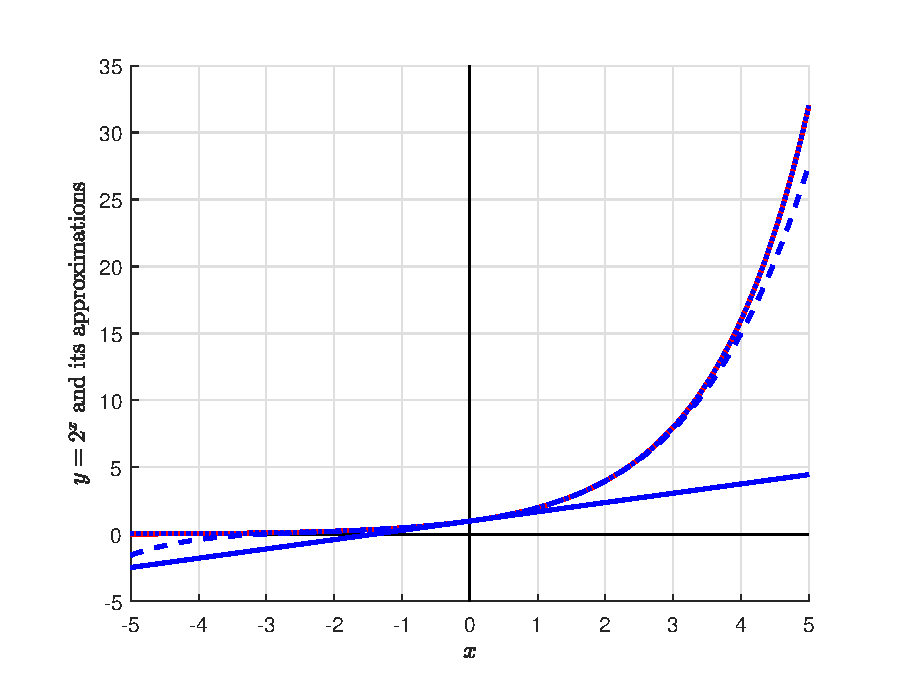
\includegraphics[width=250pt]{chapters/part-1/figures/taylorseriesexp.eps}
\caption{Plot of function $y=2^x$ in red solid line, and its approximations using first-order, $5$th-order and $10$th-order Taylor series in blue solid line, blue dashed line and blue dot line respectively.} \label{ch4fig:taylordemo}
\end{figure}

For polynomial functions $f(x)$, $f^{(n)}(x) = 0$ for large enough $n$, depending on the degree of the polynomial. For a $N$-th-order polynomial, $f^{(n)}(x) = 0$ for $n>N$, thus its $n$-th-order (or higher) Taylor series $P(x,x_0)=f(x)$ for any choice of $x_0$.
